% Created by tikzDevice version 0.12.6 on 2026-09-11 15:07:16
% !TEX encoding = UTF-8 Unicode
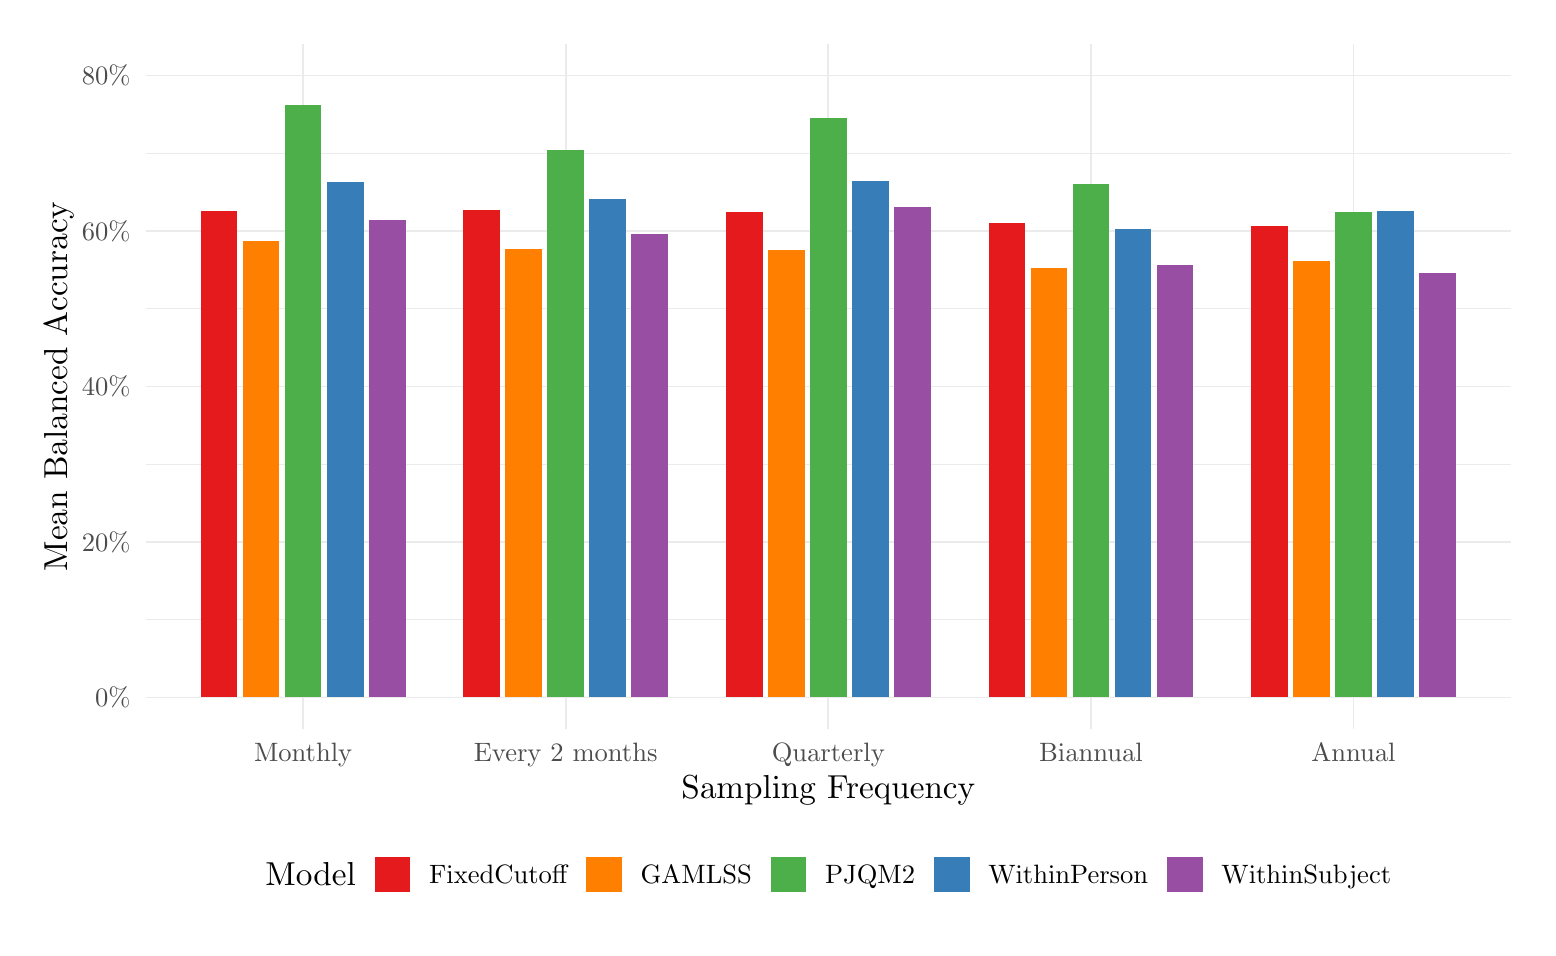
\begin{tikzpicture}[x=1pt,y=1pt]
\definecolor{fillColor}{RGB}{255,255,255}
\path[use as bounding box,fill=fillColor,fill opacity=0.00] (0,0) rectangle (542.02,325.21);
\begin{scope}
\path[clip] (  0.00,  0.00) rectangle (542.02,325.21);
\definecolor{fillColor}{RGB}{255,255,255}

\path[fill=fillColor] (  0.00,  0.00) rectangle (542.02,325.21);
\end{scope}
\begin{scope}
\path[clip] ( 42.59, 71.93) rectangle (536.03,319.21);
\definecolor{drawColor}{gray}{0.92}

\path[draw=drawColor,line width= 0.3pt,line join=round] ( 42.59,111.27) --
	(536.03,111.27);

\path[draw=drawColor,line width= 0.3pt,line join=round] ( 42.59,167.47) --
	(536.03,167.47);

\path[draw=drawColor,line width= 0.3pt,line join=round] ( 42.59,223.67) --
	(536.03,223.67);

\path[draw=drawColor,line width= 0.3pt,line join=round] ( 42.59,279.87) --
	(536.03,279.87);

\path[draw=drawColor,line width= 0.6pt,line join=round] ( 42.59, 83.17) --
	(536.03, 83.17);

\path[draw=drawColor,line width= 0.6pt,line join=round] ( 42.59,139.37) --
	(536.03,139.37);

\path[draw=drawColor,line width= 0.6pt,line join=round] ( 42.59,195.57) --
	(536.03,195.57);

\path[draw=drawColor,line width= 0.6pt,line join=round] ( 42.59,251.77) --
	(536.03,251.77);

\path[draw=drawColor,line width= 0.6pt,line join=round] ( 42.59,307.97) --
	(536.03,307.97);

\path[draw=drawColor,line width= 0.6pt,line join=round] ( 99.53, 71.93) --
	( 99.53,319.21);

\path[draw=drawColor,line width= 0.6pt,line join=round] (194.42, 71.93) --
	(194.42,319.21);

\path[draw=drawColor,line width= 0.6pt,line join=round] (289.31, 71.93) --
	(289.31,319.21);

\path[draw=drawColor,line width= 0.6pt,line join=round] (384.20, 71.93) --
	(384.20,319.21);

\path[draw=drawColor,line width= 0.6pt,line join=round] (479.09, 71.93) --
	(479.09,319.21);
\definecolor{fillColor}{RGB}{228,26,28}

\path[fill=fillColor] ( 62.52, 83.17) rectangle ( 75.80,258.92);

\path[fill=fillColor] (157.41, 83.17) rectangle (170.70,259.38);

\path[fill=fillColor] (252.30, 83.17) rectangle (265.59,258.44);

\path[fill=fillColor] (347.19, 83.17) rectangle (360.48,254.56);

\path[fill=fillColor] (442.08, 83.17) rectangle (455.37,253.55);
\definecolor{fillColor}{RGB}{255,127,0}

\path[fill=fillColor] ( 77.70, 83.17) rectangle ( 90.99,248.01);

\path[fill=fillColor] (172.59, 83.17) rectangle (185.88,245.11);

\path[fill=fillColor] (267.48, 83.17) rectangle (280.77,244.82);

\path[fill=fillColor] (362.37, 83.17) rectangle (375.66,238.31);

\path[fill=fillColor] (457.27, 83.17) rectangle (470.55,240.93);
\definecolor{fillColor}{RGB}{77,175,74}

\path[fill=fillColor] ( 92.89, 83.17) rectangle (106.17,297.13);

\path[fill=fillColor] (187.78, 83.17) rectangle (201.06,280.92);

\path[fill=fillColor] (282.67, 83.17) rectangle (295.95,292.46);

\path[fill=fillColor] (377.56, 83.17) rectangle (390.84,268.79);

\path[fill=fillColor] (472.45, 83.17) rectangle (485.73,258.68);
\definecolor{fillColor}{RGB}{55,126,184}

\path[fill=fillColor] (108.07, 83.17) rectangle (121.35,269.50);

\path[fill=fillColor] (202.96, 83.17) rectangle (216.24,263.28);

\path[fill=fillColor] (297.85, 83.17) rectangle (311.13,269.91);

\path[fill=fillColor] (392.74, 83.17) rectangle (406.02,252.59);

\path[fill=fillColor] (487.63, 83.17) rectangle (500.92,259.09);
\definecolor{fillColor}{RGB}{152,78,163}

\path[fill=fillColor] (123.25, 83.17) rectangle (136.54,255.60);

\path[fill=fillColor] (218.14, 83.17) rectangle (231.43,250.63);

\path[fill=fillColor] (313.03, 83.17) rectangle (326.32,260.47);

\path[fill=fillColor] (407.92, 83.17) rectangle (421.21,239.38);

\path[fill=fillColor] (502.81, 83.17) rectangle (516.10,236.60);
\end{scope}
\begin{scope}
\path[clip] (  0.00,  0.00) rectangle (542.02,325.21);
\definecolor{drawColor}{gray}{0.30}

\node[text=drawColor,anchor=base east,inner sep=0pt, outer sep=0pt, scale=  0.96] at ( 37.19, 79.86) {0\%};

\node[text=drawColor,anchor=base east,inner sep=0pt, outer sep=0pt, scale=  0.96] at ( 37.19,136.07) {20\%};

\node[text=drawColor,anchor=base east,inner sep=0pt, outer sep=0pt, scale=  0.96] at ( 37.19,192.27) {40\%};

\node[text=drawColor,anchor=base east,inner sep=0pt, outer sep=0pt, scale=  0.96] at ( 37.19,248.47) {60\%};

\node[text=drawColor,anchor=base east,inner sep=0pt, outer sep=0pt, scale=  0.96] at ( 37.19,304.67) {80\%};
\end{scope}
\begin{scope}
\path[clip] (  0.00,  0.00) rectangle (542.02,325.21);
\definecolor{drawColor}{gray}{0.30}

\node[text=drawColor,anchor=base,inner sep=0pt, outer sep=0pt, scale=  0.96] at ( 99.53, 59.92) {Monthly};

\node[text=drawColor,anchor=base,inner sep=0pt, outer sep=0pt, scale=  0.96] at (194.42, 59.92) {Every 2 months};

\node[text=drawColor,anchor=base,inner sep=0pt, outer sep=0pt, scale=  0.96] at (289.31, 59.92) {Quarterly};

\node[text=drawColor,anchor=base,inner sep=0pt, outer sep=0pt, scale=  0.96] at (384.20, 59.92) {Biannual};

\node[text=drawColor,anchor=base,inner sep=0pt, outer sep=0pt, scale=  0.96] at (479.09, 59.92) {Annual};
\end{scope}
\begin{scope}
\path[clip] (  0.00,  0.00) rectangle (542.02,325.21);
\definecolor{drawColor}{RGB}{0,0,0}

\node[text=drawColor,anchor=base,inner sep=0pt, outer sep=0pt, scale=  1.20] at (289.31, 46.79) {Sampling Frequency};
\end{scope}
\begin{scope}
\path[clip] (  0.00,  0.00) rectangle (542.02,325.21);
\definecolor{drawColor}{RGB}{0,0,0}

\node[text=drawColor,rotate= 90.00,anchor=base,inner sep=0pt, outer sep=0pt, scale=  1.20] at ( 14.26,195.57) {Mean Balanced Accuracy};
\end{scope}
\begin{scope}
\path[clip] (  0.00,  0.00) rectangle (542.02,325.21);
\definecolor{drawColor}{RGB}{0,0,0}

\node[text=drawColor,anchor=base west,inner sep=0pt, outer sep=0pt, scale=  1.20] at ( 85.93, 15.09) {Model};
\end{scope}
\begin{scope}
\path[clip] (  0.00,  0.00) rectangle (542.02,325.21);
\definecolor{fillColor}{RGB}{228,26,28}

\path[fill=fillColor] (125.37, 12.78) rectangle (138.27, 25.68);
\end{scope}
\begin{scope}
\path[clip] (  0.00,  0.00) rectangle (542.02,325.21);
\definecolor{fillColor}{RGB}{255,127,0}

\path[fill=fillColor] (201.81, 12.78) rectangle (214.71, 25.68);
\end{scope}
\begin{scope}
\path[clip] (  0.00,  0.00) rectangle (542.02,325.21);
\definecolor{fillColor}{RGB}{77,175,74}

\path[fill=fillColor] (268.45, 12.78) rectangle (281.36, 25.68);
\end{scope}
\begin{scope}
\path[clip] (  0.00,  0.00) rectangle (542.02,325.21);
\definecolor{fillColor}{RGB}{55,126,184}

\path[fill=fillColor] (327.43, 12.78) rectangle (340.34, 25.68);
\end{scope}
\begin{scope}
\path[clip] (  0.00,  0.00) rectangle (542.02,325.21);
\definecolor{fillColor}{RGB}{152,78,163}

\path[fill=fillColor] (411.69, 12.78) rectangle (424.59, 25.68);
\end{scope}
\begin{scope}
\path[clip] (  0.00,  0.00) rectangle (542.02,325.21);
\definecolor{drawColor}{RGB}{0,0,0}

\node[text=drawColor,anchor=base west,inner sep=0pt, outer sep=0pt, scale=  0.96] at (145.05, 15.92) {FixedCutoff};
\end{scope}
\begin{scope}
\path[clip] (  0.00,  0.00) rectangle (542.02,325.21);
\definecolor{drawColor}{RGB}{0,0,0}

\node[text=drawColor,anchor=base west,inner sep=0pt, outer sep=0pt, scale=  0.96] at (221.49, 15.92) {GAMLSS};
\end{scope}
\begin{scope}
\path[clip] (  0.00,  0.00) rectangle (542.02,325.21);
\definecolor{drawColor}{RGB}{0,0,0}

\node[text=drawColor,anchor=base west,inner sep=0pt, outer sep=0pt, scale=  0.96] at (288.13, 15.92) {PJQM2};
\end{scope}
\begin{scope}
\path[clip] (  0.00,  0.00) rectangle (542.02,325.21);
\definecolor{drawColor}{RGB}{0,0,0}

\node[text=drawColor,anchor=base west,inner sep=0pt, outer sep=0pt, scale=  0.96] at (347.11, 15.92) {WithinPerson};
\end{scope}
\begin{scope}
\path[clip] (  0.00,  0.00) rectangle (542.02,325.21);
\definecolor{drawColor}{RGB}{0,0,0}

\node[text=drawColor,anchor=base west,inner sep=0pt, outer sep=0pt, scale=  0.96] at (431.37, 15.92) {WithinSubject};
\end{scope}
\end{tikzpicture}
